\chapter{Ferdinand de Saussure}
\label{ch.saussure_life}\

Conventional wisdom holds that the distinctive content of twentieth
century linguistics can in large part be traced back to the work of
the Genevan linguist \name{Ferdinand}{de Saussure}.  To be sure, the
literature displays a certain amount of jostling for position with
regard to historical priority on particular points or the possible
influences exerted on {\Saussure} by others; furthermore, the details of
just how {\Saussure} acquired (or rather was given) such an influential
status remain quite obscure
\citep{percival77:rvw.koerner.saussure}. Nonetheless, it seems almost
universally agreed that {\Saussure}'s views establish a genuine
milestone, and the beginnings of what we think of as the modern
approach to the study of language.

Nonetheless, it is not always easy for those who come to the
\textsl{Cours de linguistique g\'en\'erale} \citep{saussure:cours} for
the first time to see just what all the fuss is about. Many of the
observations that seem to form the core of {\Saussure}'s system appear
thoroughly obvious to the modern reader (when they are not quaintly
obscure!), and it is not especially obvious why this should have been
such an important book.  The reason for this reaction is not simply
that {\Saussure}'s views have now become the accepted starting point for
the field, and are thus familiar: after all, we can appreciate the
innovative nature of Copernican astronomy even though its basic
results are by now common knowledge. Rather, the difficulty we have in
understanding the importance of {\Saussure}'s views may be traced to
their apparent obviousness in a completely pre-scientific sense.  One
has to be an astronomer, with specialized equipment and mathematical
techniques at one's disposal in order to make and interpret the
observations that lead to the conclusion that the planets rotate
around the sun rather than \emph{vice versa}, but it seems that anyone
at all should be able to see the difference between a language as a
system and speech as behavior, between the historical development of a
language and its present state, and other cornerstones of Saussurean
theory.

Indeed, many of his observations obviously had been made before by
others, and {\Saussure}'s importance does not rest on the claim that
everything he said was totally original.  Rather, he brought a lot of
observations together into a unified system quite at variance with the
theories then current in the scientific study of language.  Despite
their apparent self-evidence, we must realize that {\Saussure}'s basic
premises were (in their historical context) thoroughly opposed to
those underlying the way scientific linguistics was then being carried
out.  Furthermore, the very obviousness of many of {\Saussure}'s
propositions, taken individually, lends the resulting totality a kind
of immediacy that accounts for its persuasive (and ultimately
revolutionary) character.

{\Saussure}'s own view of the importance of his enterprise was that he
posed the basic question of \emph{what a language is}, and held it to
be the fundamental responsibility of linguistics to provide an answer.
Although it may seem self-evident that this is what linguistics is
about, we have to recognize that at the time, it marked a really basic
shift in attitude.  Others had taken it for granted, that is, that
everyone knows what a language \emph{is}, and that the questions
suitable for scientific study are such as: how do natural languages
evolve and change?  where did language come from in the first place?
how is logical thought reflected in the structure of language?  etc.
The demonstrated successes of 19th century comparative linguistics had
focused nearly all of the scientific attention that was devoted to
language on issues quite distinct from the essential character of
linguistic systems, and it was {\Saussure}'s accomplishment largely to
reverse this trend.  As a result, and without denying the continuing
importance of the study of linguistic change, post-Saussurean
linguistics has been primarily devoted to synchronic, theoretical
studies that are based (at least in principle) on descriptions of
actual \emph{états de langue}.

In {\Saussure}'s view, the serious study of language might be thought to
have begun with the tradition of medieval speculative or philosophical
grammar.  This evolved, however, into (what he saw as) merely
prescriptive studies, concerned not with what the system of a
particular language is, but rather with what it ought to be.  Then in
the 19th century, the growing success of comparative linguistics
shifted attention to the question of where particular language states
come from.  This view purported to provide an {explanation} of any given
language in terms of its past; but since it resolutely denied the
possibility of finding {explanation} in any specific present state of
affairs, it resulted in an even greater diversion of linguists'
energies away from the task of accounting for the basic problem of
what a language \emph{is}.

{\Saussure} thus called for a refounding of the essentially synchronic
study of language (note that it is difficult even to state this point
without using the Saussurean vocabulary), on the basis of a search for
{explanation} and for insight into the fundamental character of the
object of study. On this basis alone, his place in the history of the
field would surely be guaranteed.  More than this, however, and in a
more detailed way, {\Saussure} initiated the focus which has dominated
the field since on languages as \emph{systems} (as his student {\Meillet}
put it, ``\emph{où tout se tient}''), rather than on the often
atomistic study of particular elements.  Much of the success of
historical linguistic studies had come from concentrating attention on
the histories of individual sounds (or limited groups of similar
sounds); {\Saussure} held out the hope that such a piecemeal (and
ultimately fragmented) approach was not the only possible path to a
genuinely scientific study of human language.

If a narrow focus on particulars loses sight of the systematic
structure within which they find their linguistic place, the attempt
to embrace all aspects of the phenomenon of  `Language' in a single
unified inquiry is also unsatisfactory, since it cannot fail to lead
to incoherence.  ``Taken in its entirety, language is multiform and
irregular; straddling several domains, simultaneously physical,
physiological and psychological, it belongs both to the individual and
to the social realm; it cannot be classified within any category of
human reality, because there is no way to distinguish its unity''
(\textsl{Cours de linguistique générale}, p.  25, my translation).
The answer to this dilemma is quite simply to focus on the aspect of
language that does furnish a unitary object of inquiry: the nature of
the underlying systems of particular languages.  His work thus did
nothing less than establish the fundamental character of the
discipline since then.

\section{Saussure's life and career}


For linguists, \name{Ferdinand}{de Saussure} stands as a dominating figure of
great historical
significance.\footnote{\protect\citet{joseph12:saussure} provides a
  richly detailed description of \name{Ferdinand}{de Saussure}'s family
  background, his life, and the social, intellectual and professional
  context of his career, from which some of the account below is
  derived.} It is therefore somewhat surprising to realize that in
Geneva (where he was born and where he spent the majority of his
academic life), he is by no means the figure that comes first to mind
in connection with the name de Saussure. In fact, his family was one
that was quite important in scientific and intellectual circles in
Switzerland well before his birth in 1857, and other de Saussures have
been more prominent in Swiss history and {culture}.  His great-uncle
\name{Horace-Bénédict}{de Saussure} (1740-1799) in particular was a major
figure in the development of the natural sciences in Geneva; he was
especially celebrated for observations made on one of the first
ascensions of Mont Blanc, which still form a basis for map-making in
Switzerland.  A number of other ancestors, dating at least to the
beginning of the 18th century, played \isi{significant} roles in a variety
of scientific fields.

As a result of his family background, it was hardly surprising that
the young \name{Ferdinand}{de Saussure} was sent to the newly organized
University of Geneva in 1875, with the hope that he would study
physics and chemistry.  He seems to have discovered early on that he
was more interested in pursuing linguistic studies than in physics and
chemistry, and in fact ended his study of these subjects somewhat
disastrously, to the distress of his father.

By this time he had studied (besides {French} and {German}) {English},
{Latin}, and {Greek}; and indeed at the age of 15 he had written an essay
on the reduction of all languages to a system of two or three basic
\isi{consonants}. During his year at the University of Geneva he enrolled in
a bewildering variety of courses in addition to those in the sciences,
and in the end had less to show for it than he or his family might
have wished. He did, however, produce a paper (on the suffix
\emph{-t-} in \ili{Indo-European}, \citealt{saussure77:suffix.t}), which he
submitted to the Société de Linguistique de Paris in support of his
application for membership. When this was accepted for
publication in the society's \emph{Mémoires,} that success at least
partially redeemed him in his father's estimation.

\begin{wrapfigure}[14]{l}{.4\textwidth}
  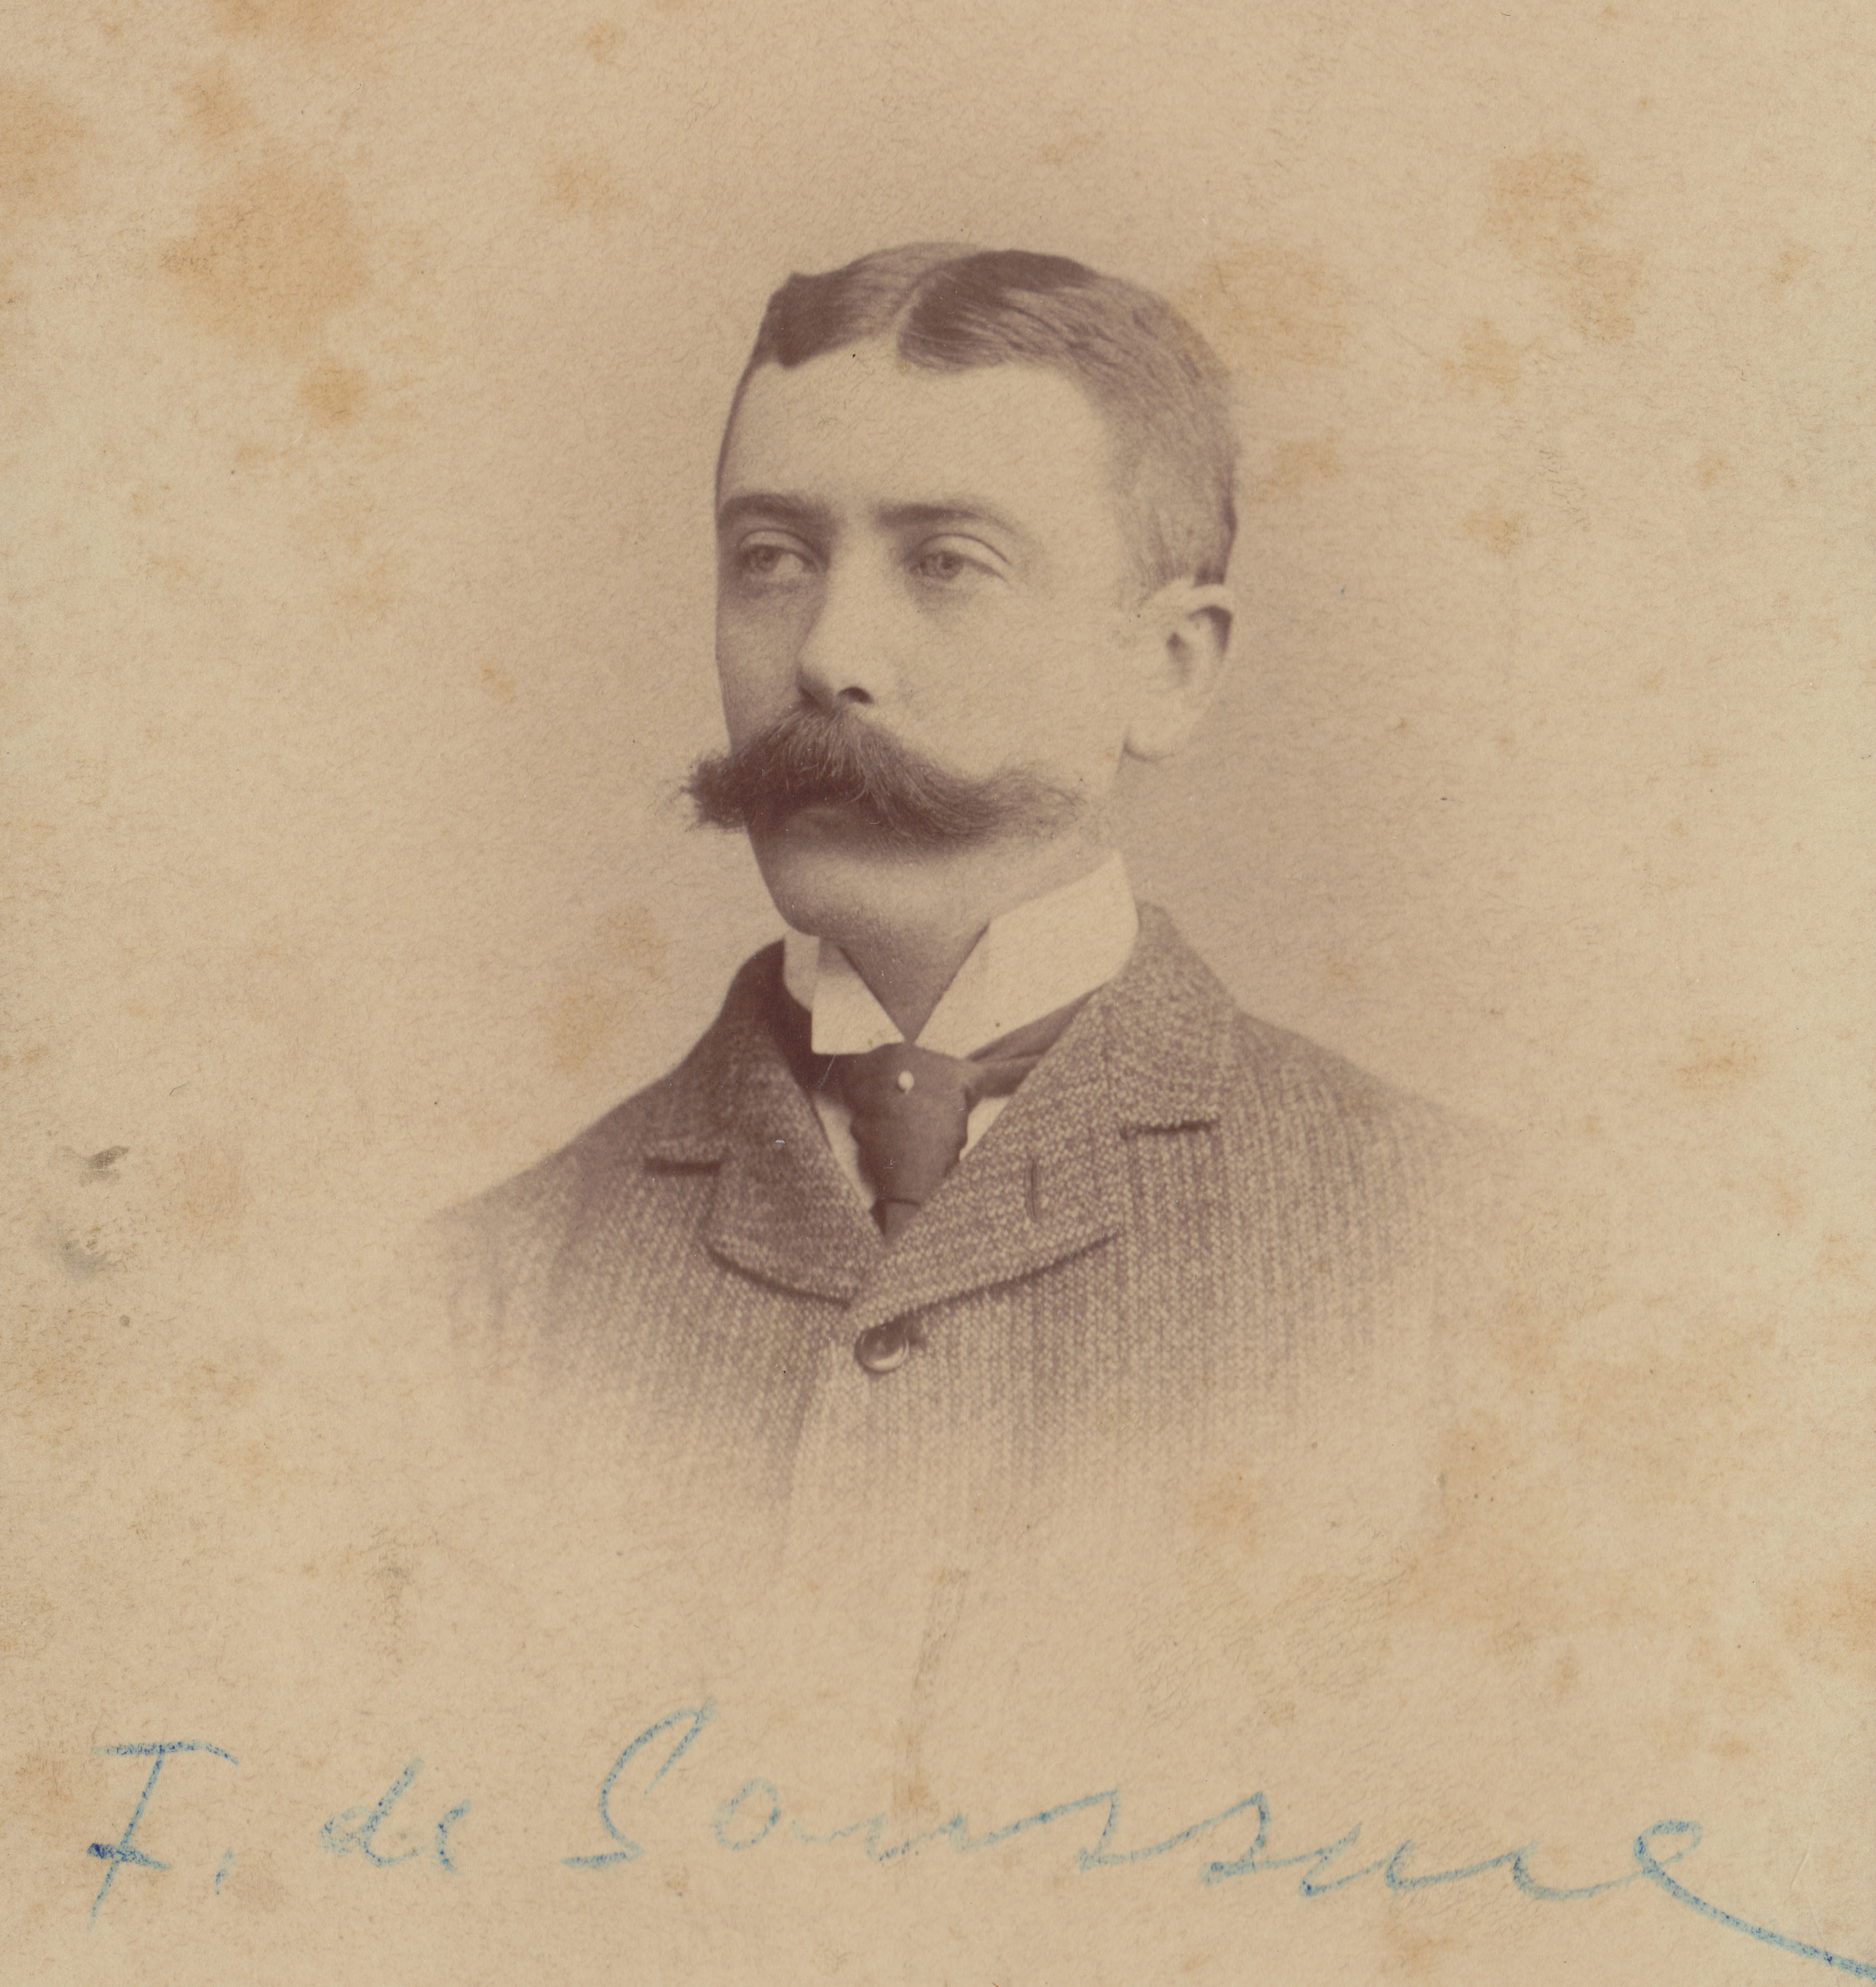
\includegraphics[width=.9\textwidth]{figures/Young_Saussure.jpg}
  \caption{Ferdinand de Saussure as a young man}
  \label{fig:ch.saussure_life.young_saussure}
\end{wrapfigure}
In 1876 his father, giving up on his hopes that Ferdinand {\Saussure} would follow
in the family's tradition of work in the sciences, took him to {Leipzig}
to study \ili{Indo-European} with such figures as \name{Georg}{Curtius}, \name{Wilhelm}{Braune}, \name{Hermann}{Osthoff} and \name{August}{Leskien}. {Leipzig}'s linguistic
luminaries also included \name{Karl}{Brugmann}, with whom his relationship was
initially somewhat prickly and never completely resolved.  This was in
part as a result of lingering resentment over matters of research
priority, especially for the theory of syllabic nasals in
\ili{Indo-European}; the young Saussure had arrived at essentially the same
conclusions as {\Brugmann} some years earlier, but simply assumed that
this would be common knowledge among serious students of
\ili{Indo-European}. He was thus somewhat surprised to learn that {\Brugmann}'s
announcement of a relation between the nasal \emph{n} and the vowel
\emph{a} was being taken as revolutionary in {Leipzig}. The next four
years (with the exception of a year and a half studying {Sanskrit} and
Celtic in Berlin) were to be spent among the {Leipzig}
`\isi{Junggrammatiker}.'

1876 was a particularly \isi{significant} year to arrive in {Leipzig}: this is
generally considered the year in which, with regard to the developing
theory of the Neo\-grammarians, ``everything seemed to happen at once''
\citep{hoenigswald78:annus.mirabilis}. This was the year in which,
among other things, {\Leskien} formulated the doctrine of the regularity
of \isi{sound change}, {\Verner} published his famous article on exceptions to
Grimm's law, {\Brugmann} presented his theory of the syllabic nasals; and
{\Sievers} published his \textsl{Grundz\"uge der Lautphysiologie}
(\citealt{sievers76:lautphysiologie}, later revised as
\citealt{sievers:phonetik}) which established the phonetic
underpinnings of the theory of \isi{sound change}.  {\Saussure} was thus
immediately caught up in the sort of atmosphere that surrounds
scientific revolutions.

His previous time spent studying languages and thinking about general
problems in linguistics had evidently prepared him well to participate
actively in this work. He had already in 1875 been admitted to
membership in the Société de Linguistique de Paris, and his paper on
the suffix \emph{-t-} appeared in its journal.  Several other short
papers followed. His major work, however, was
\citet{saussure:memoire}, the monumental \textsl{Mémoire sur le
  système primitif des voyelles dans les langues indo-européennes},
which appeared in {Leipzig} in December, 1878 (though the first edition
bears the date 1879).

The influence of this work, which presented a comprehensive
reconstruction of the vocalic system of \ili{Indo-European}, is hard to
exaggerate: it is by no means absurd to compare its influence on
\ili{Indo-European} linguistics with the influence of the \textsl{Cours de
  linguistique générale} on general linguistics.  While the
process was long and slow (and indeed, one could argue that it is
still not complete), the gradual absorption into the field of
historical linguistics of the point of view in {\Saussure}'s
\textsl{Mémoire} came to determine more or less completely the
directions taken by the field.  It presented a coherent picture of
Proto-\ili{Indo-European} as a system, and defined in an innovative way the
problems which would occupy subsequent research.

The most famous aspect of this system was the theory of
`\emph{coefficients sonantiques}'; these were the elements, like
the liquids and nasals and the high vowels and semi-vowels (i/y, u/w),
which could be realized either as vowels (when surrounded by
\isi{consonants}) or as \isi{consonants} (when preceded by a vowel).  Much of the
originality and coherence of {\Saussure}'s proposal resulted from the
fact that he included in the inventory of \emph{coefficients} two
elements which (at the time) were not ever attested phonetically in a
straightforward fashion: they appeared only as some other vowel, or
else through their influence on a preceding vowel.

These, of course, were the elements which would subsequently be called
`\isi{laryngeals},' and the discovery nearly fifty years later by
\citet{kurylowicz27:hittite} of direct (consonantal) reflexes of these segments in
\ili{Hittite} was generally considered as a striking confirmation of a
brilliant conjecture on {\Saussure}'s part.  The most important aspect of
the `\isi{laryngeals}' in the \textsl{Mémoire}, however, was not the
discovery of some additional Proto-\ili{Indo-European} segments, but rather
the methodology which led {\Saussure} to posit them.  It was precisely by
considering the \ili{Indo-European} sonants \emph{as a system} that he
was led to conclude the existence of additional elements which, though
not directly attested (as \isi{consonants}), nonetheless behaved according
to the {rules} of the system, and whose effects were apparent in the
attested forms. This point of view, which seeks the coherence of the
system constituted by a language (whether that language is observed
directly or reconstructed) rather than simply investigating the
history of the individual elements comprising the system, was quite
different from the dominant line in historical studies at the time.
Partly on its own, and partly because of the dramatic success of the
`laryngeal theory,' however, it has come to underlie most modern
serious work in historical as well as general linguistics.

There is a reasonably direct connection between the \textsl{Mémoire}
and {\Saussure}'s later views on language, in the extent to which the
notion of a \isi{linguistic system} (as opposed to a simple inventory of
elements) plays a central role in his work throughout.  His
development in connection with his \ili{Indo-European} studies of a rather
elaborate theory of the structure of syllables and their importance
for phonetics constitutes another link between this work and his other
writing. The picture of phonetic structure that would later be
developed (and presented slightly out of context by his editors) in
the \textsl{Cours} is based on the notion that the actual phonetic
value of a segment is a function of a) its ``phonetic species''
(roughly, its basic articulatory/acoustic type, characterized e.g. as
a static position of the articulatory organs) and b) its position in
the \isi{syllable} (or perhaps in larger units in the spoken chain).  We
will return below in chapter~\ref{ch.saussure_sound} to the substance
of {\Saussure}'s views on such issues of \isi{sound structure}; for now we can
simply note a connection between the phonetic presentation in the
\textsl{Cours} and the issues dealt with in the \textsl{Mémoire}
(especially the nature of the \emph{coefficients sonantiques}, whose
realization is essentially dependent on the role they play in \isi{syllable}
structure).

In {contrast} with the vast range of the \textsl{Mémoire}, the
dissertation which {\Saussure} presented in 1880
\citep{saussure81:dissertation} for his doctorate in {Leipzig} seems
remarkably limited. This dealt with the uses of the genitive absolute
construction in \ili{Sanskrit}. He seems to have chosen the topic in part
because it lay as far as possible from the subject of the
\textsl{Mémoire}, whose reception by at least some of the
\isi{Leipzig} linguists was somewhat hostile --- an attitude he feared might
compromise his chances of obtaining the doctorate. While there is no
question that the thesis was an extremely learned work, the efforts of
later Saussure scholars to identify fundamental issues of linguistic
structure addressed in it have not been notably successful.  Its merit
(and the mention `\emph{egregia}' --- \emph{summa cum laude} which
{\Saussure} received at his defense) rested much more on a display of
erudition than on lasting significance.

With respect to his published work, indeed, the \textsl{Mémoire} was
nearly the only important thing {\Saussure} ever wrote.  During the ten
years after his doctoral thesis, he produced several comparatively
short articles devoted to particular historical problems in individual
languages.  Probably the most \isi{significant} of these dealt with the
accentual system of \ili{Lithuanian},\footnote{See
  \citealt{joseph09:saussure.lithuanian} for discussion.} but it seems
that even here, only a part of what he had to say ever appeared in
print.  And for the rest of his life, he would produce virtually
nothing more in written form.

Following his doctorate in 1880, {\Saussure} left {Leipzig} (where a
certain amount of tension had entered into his relations with the
\emph{Junggrammatiker}) for Paris, after a brief stay in
Lithuania. Here he followed a few courses and became quite active in
the Société linguistique.  By the fall of 1881, he was appointed as
the equivalent\footnote{Since {\Saussure} was not a {French} citizen, his
  eligibility for formal academic appointments in a {French} university
  was limited at the time.} of Lecturer, `\emph{maître de conférences
  de gothique et de vieux-haut allemand}' at the \emph{École Pratique
  des Hautes Études}. For the next ten years he taught a series of
courses there, primarily in {Germanic}, but including also {Greek} and
{Latin} in 1887--8, and more general considerations of {Indo-European}
structure in his last years in Paris.

His were among the most important courses being offered in historical
linguistics in Paris, and over time he attracted a comparatively large
number of students --- many of them, apparently, quite good
(including, e.g., \name{Antoine}{Meillet}, \name{Maurice}{Grammont}, \name{Paul}{Passy}, and
others whose influence would later be fundamental in the field).
During these years he was also much occupied with the affiars of the
Société linguistique, regularly attending its meetings, giving and
commenting on papers, and serving in the important administrative role
of Adjunct Secretary, with responsibility for the Society's
publications. Partly as a result of this activity, he was in direct
contact with most of the major linguists of the time, not only the
\ili{French}.

His career in Paris seemed to offer great promise. On the strength of
the \textsl{Mémoire} he was seen as a major intellectual force in
\ili{Indo-European} studies. A combination of personal and professional
setbacks, however, together with his failure to produce any work of
comparable significance in subsequent years, served to constrain his
chances of real success.  When a chair in \ili{Sanskrit} and Comparative
\ili{Indo-European} unexpectedly fell vacant, he might well have been the
natural person to be appointed to it, but this did not happen, and the
resulting disappointment rather soured him on his prospects in the
academic world of Paris.

Efforts were being made to persuade him to return to Geneva, and in
the course of the academic year 1890-91 he decided to resign his
position in Paris. Before leaving he was named a \emph{Chevalier de la
  Légion d'Honneur}, and some of his Paris colleagues apparently hoped
he might return at some point in the future.  Nonetheless, he decided
in that year to leave Paris and return to Geneva.

\begin{wrapfigure}{r}{.4\textwidth}
  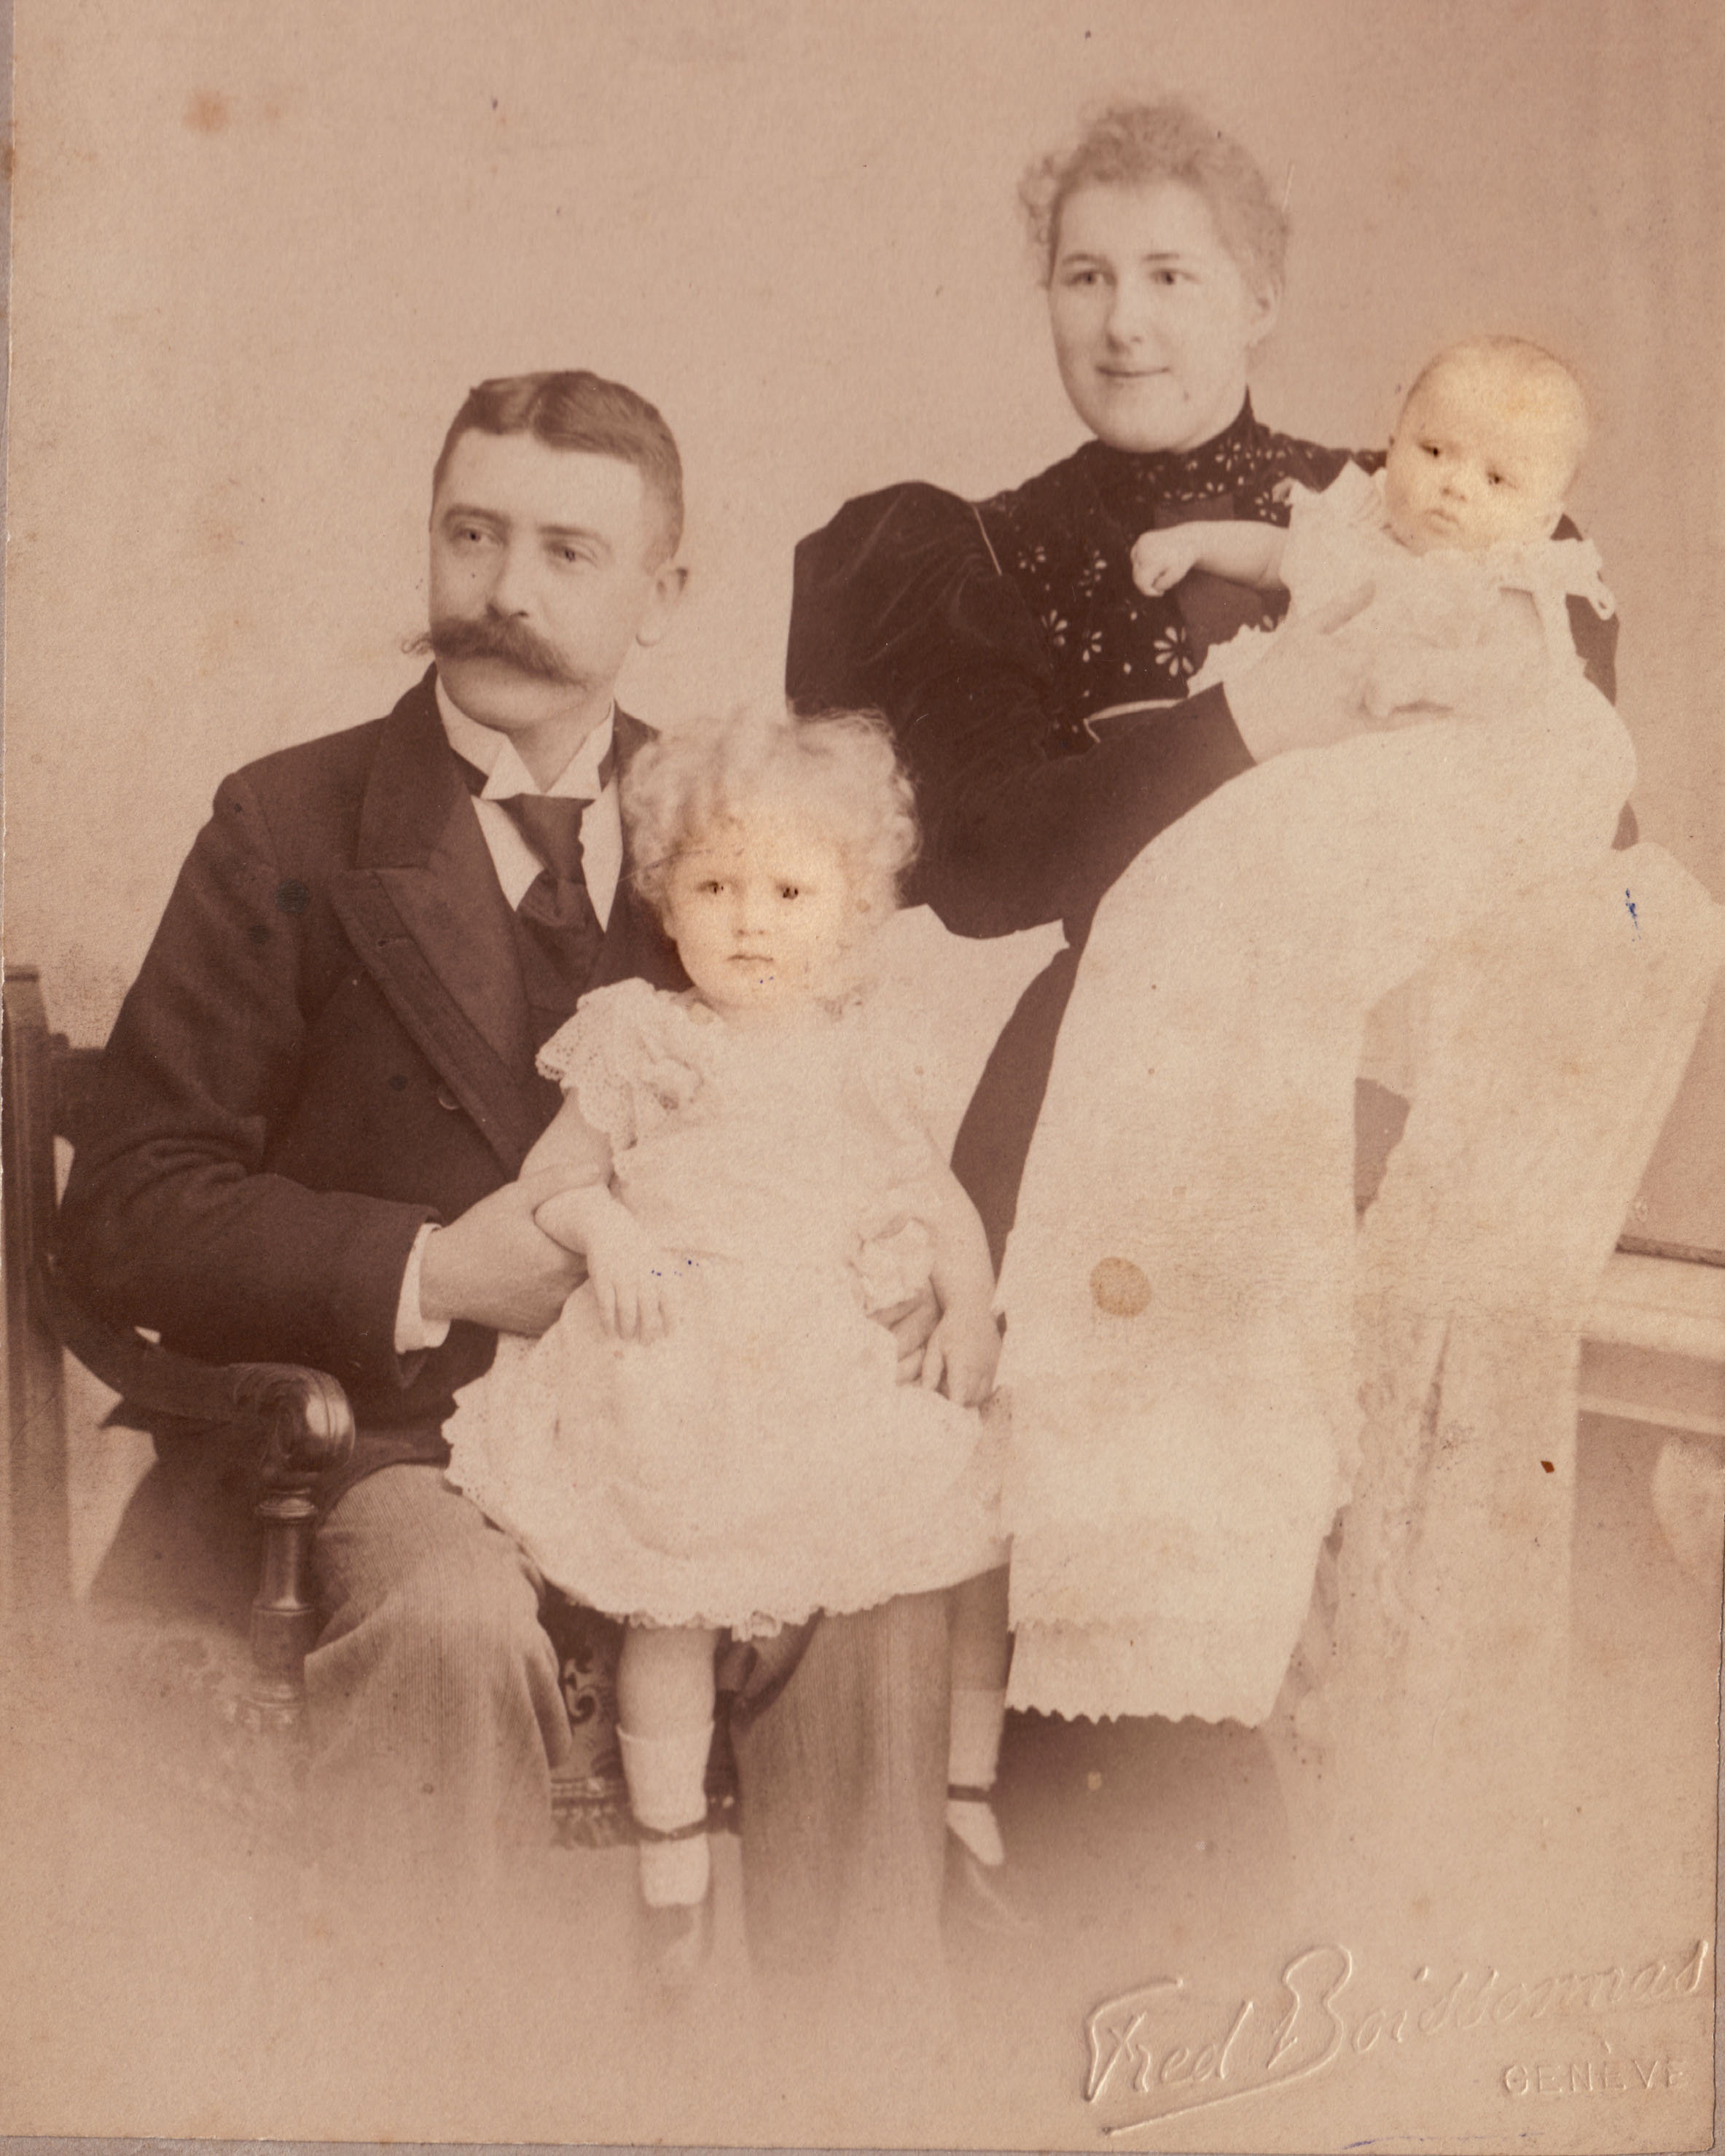
\includegraphics[width=.9\textwidth]{figures/DeSaussure_and_family.jpg}
  \caption{Ferdinand de Saussure with his wife Marie and sons Jacques [l.]
    and Raymond [r.]}
  \label{fig:ch.saussure_life.saussure_family}
\end{wrapfigure}
While in Paris, he had hoped to marry the daughter of a prominent
{French} family, \name{Noémi}{Mallet}, but this possibility disappeared with his
failure to obtain a professorial chair. Shortly after his return to
Switzerland, in March, 1892, {\Saussure} was married to the daughter of a
family friend, \name{Marie-Eugénie}{Faesch}. They had two sons Jacques and
Raymond (Figure~\ref{fig:ch.saussure_life.saussure_family}); a third
son André died at the age of three months in 1895.

In Geneva, a chair was created for {\Saussure} as \emph{Professeur
  extaordinaire}, to teach {Sanskrit} and {Indo-European}.  For the next
22 years, until his death in 1913, he taught in Geneva, where his
students were many fewer and much less prepared. Indeed, with the
exception of a few foreign students who came to Geneva specifically to
study with him (such as S. {\Karcevskij}), it is probably not unfair to
suggest that hardly any of them achieved distinction in any area
except the chronicling of {\Saussure}'s life during this time.

His written output, too (already rather sparse during his years in
Paris), came to a virtual standstill. In part this seems to have
reflected a general disenchantment on his part with the conceptual
bases of the field of linguistics.  In a letter to {\Meillet} (from 1894,
quoted by \citet[31]{godel57:sources}), for instance, he says that he
could not write anything sensible about the languages he was working
on because it would be necessary first to undertake the immense task
of showing linguists just what it is they do: i.e., to reconsider the
very foundations of our conception of language.  

In any event, he was assigned (in 1906, on the death of another
Professor) responsibility for courses in general linguistics as well
as his basic classes in {Sanskrit} and {Indo-European}, and the lectures
that resulted have largely formed the basis of {\Saussure}'s reputation
since. On three occasions (in 1907, 1908--9, and 1910--11), {\Saussure}
gave a course in general linguistics at the University of Geneva.
When he died in 1913, he had not written any of this material in
publishable form; indeed, he had destroyed the greater part of his
lecture notes.  As a result, we would be left with little but the
reminiscences of his students if it were not for the activity
undertaken by two of his colleagues.

\name{Charles}{Bally} and \name{Albert}{Sechehaye} had not in fact attended {\Saussure}'s
lectures on general linguistics, but were generally familiar with the
position that had been presented in them (Mrs.  Sechehaye, indeed, had
been one of the students in {\Saussure}'s third and last series of
lectures\footnote{Lectures published with {English} translation as
  \citealt{saussure93:troisieme-cours} on the basis of notes by
  another student.  These notebooks are published in a more complete
  form as \citealt{constantin05:troisieme-cours} together with several
  articles on the text in the same volume of \textsl{Cahiers Ferdinand
    de Saussure}.}).  They undertook, after his death, to reconstruct
a book which {\Saussure} \emph{might} have written, on the basis of the
little manuscript material that was available and, primarily, the
notes taken by students in his lectures. The resulting \textsl{Cours
  de linguistique générale} was published as
\citealt{saussure16:cours-original}, and it is this work which is
generally referred to when one asserts that ``Saussure said'' thus and
so. The consequence of this method by which ``Saussure's'' work was
prepared for publication is that we have very little direct evidence
for what {\Saussure} actually said about most things, although the
consistency of the student notes used by {\Bally} and {\Sechehaye}, together
with the unpublished material which they and others (especially
\citet{godel54:notes,godel57:sources} and
\citet{engler68-74:edition.critique}) have provided since give us a
reasonable basis for judgment on many topics.

The indirectness of our access to {\Saussure}'s thought is curiously
appropriate, though. After a rather critical reception accorded the
first edition of the \textsl{Cours}, it gradually came to be well
known during the 1920s and 1930s, partly through translations. It is
worth noting that an {English} translation did not appear until 1959,
which is surely responsible at least in part for the general lack of
direct reference to Saussurean thought in British and American
linguistics before then (apart from a short andnot particularly
sympathetic review by \citet{bloomfield23:review-saussure} and a
rather limited presentation by \citet{wells47:saussure}).  {\Saussure}'s
influence, such as it was, was exerted almost entirely through this
book, rather than through any actual linguistic work of his own or of
his students.  This effect was almost entirely posthumous, and as a
result, his importance rests more on what people \emph{thought} he
said than on what he actually did say.  The indirect way in which the
\textsl{Cours} reflects his thought, then, helps to emphasize the
exact nature of his influence on the subsequent development of
specific areas such as phonology.

Despite the fact that {\Saussure}'s `actual' views (whatever they were)
were of less importance to the development of the field than the
version that was presented by others, we will follow much other
Saussure scholarship below in attempting to sort out what he himself
had in mind in the areas most central to phonological theory.  In
part, this enterprise is interesting in itself (and not only for
historical reasons); in part it may serve to establish some
perspective on the views others (especially those who considered
themselves to be developing a Saussurean notion of `\isi{structuralism}')
have attributed to him.

\section{The Saussurean view of language, languages, and linguistics} 

Before approaching {\Saussure}'s work in phonology \emph{per se}, we must
discuss the general view of language usually associated with the
\textsl{Cours de linguistique géné\-rale}, and therefore with
{\Saussure}.  We are concerned here to identify the overall
considerations that {\Saussure} felt were relevant to the systematic
study of language, and not specific to the study of \isi{sound structure} in
particular, which will be the subject of
chapter~\ref{ch.saussure_sound}.  If the present discussion seems
somewhat abstract and far from phonological concerns, the issues
raised here form an essential preliminary to what will follow.

A number of fundamental conceptual \isi{oppositions} form a convenient
framework for discussing {\Saussure}'s theory of language.  The most
basic (and best known) of these is the opposition between
\textbf{langue} and \textbf{parole}: roughly translatable in
\ili{English} as `language' vs. `speech,' these terms are both opposed to
\textbf{langage}, or Language in the most general sense.  As we
noted above, {\Saussure} rejects this broadly construed notion as a
coherent object of scientific inquiry, and focuses instead on the more
limited notions of \emph{langue} and \emph{parole}.

The first of these, \emph{langue}, is the aspect of language which
represents our knowledge of the systematic correspondences between
\isi{sound and meaning} that make up our language (including the knowledge
of what utterances are possible in our language, and what utterances
are not).  This `knowledge' consists for {\Saussure} of a system of
\textbf{signs} (a notion to be further explored below), each of which
can be identified with a particular association between sound and
\isi{meaning}.  This system of signs constitutes the common knowledge of a
speech community: an important aspect of it is that it is therefore
independent of the particularities of any individual member of that
community, or of any individual utterance that may be produced on a
particular occasion by a speaker of the language.

\emph{Parole}, on the other hand, is exactly the way in which this
knowledge is put to use by individual speakers on particular
occasions.  For {\Saussure}, this includes (in principle) not only the
moment-to-moment details of speaker behavior, but also the facts of
articulatory and acoustic phonetics that characterize (even in a
completely general, non speaker-dependent way) particular words in the
language.  There is a certain amount of difficulty with this notion,
as we will remark in the following chapter, but it follows in
principle from the fact that what matters to the system of
\emph{langue} is not the form taken by particular signs, but
rather the fact that these signs are distinct from one another.  Since
what is not part of \emph{langue} is part of \emph{parole}, it
follows that the phonetic form of words belongs to the latter, at
least in the concrete details of their implementation.

It will be seen that (making allowances for other differences), the
distinction between \emph{langue} and \emph{parole} is quite similar
to one which other linguists since {\Saussure} have made under other
names.  Basically, it is the difference between the system that
underlies a language (which distinguishes it for example from other
languages), and the use made of that system by the speakers of the
language on individual occasions, subject to individual limitations of
an idiosyncratic and/or situational nature. Though it is possible to
argue (endlessly, it would seem sometimes!)  about the precise extent
of the parallel, the difference between \emph{langue} and
\emph{parole} plays essentially the same role in {\Saussure}'s theory of
language as the distinction between \textbf{competence} and
\textbf{performance} in the work of {\Chomsky} and other generative
grammarians.

\emph{Competence} represents the knowledge attributed to an
(obviously non-exist\-ent) ideal speaker-hearer in a linguistically
uniform speech community and is opposed to the details of how (and to
what extent) individual speakers utilize that knowledge under
realistic conditions and subject to extra-linguistic limitations
(\emph{performance}).  Competence is thus reasonably similar in
character to {\Saussure}'s notion of \emph{langue}, making allowance
for other differences between {\Saussure}'s and Chomsky's notions of the
character of the system.  In both cases, it is this distinction that
allows the theory to ``get off the ground'' by giving a principled
basis for delimiting the object of study in a way that idealizes away
from the infinite variety of real-time events and focuses on their
systematic aspect.

The exact character of \emph{langue}, aside from its nature as a
system of mutually opposed signs, is not easy to determine with
precision from {\Saussure}'s writing.  On the one hand, \emph{langue}
is said to be intrinsically social, in that it is present in a speech
community rather than being complete in any individual. On the other
hand, it is also described on various occasions as in some way
psychological, and present in each member of the speech community.
This psychological aspect of \emph{langue} is often overlooked or
downgraded in presentations of {\Saussure}'s views, but a careful reading
of his own notes and those of his students suggests that it occupies a
more central place than is sometimes assigned to it.

It is true that there are passages in which {\Saussure} objects to a
\emph{purely} psychological interpretation of the nature of
\emph{\isi{langue}}, but these objections are evidently based on two
points.  On the one hand, \emph{langue} cannot be identified with
something psychologically present in any particular individual, since
it is the commonality of the system within a speech community that
gives it a function as a basis of communication.  This objection thus
corresponds to the idealized character of \emph{langue} mentioned
above: just as the (idealized) \isi{competence} posited by generative
grammarians is not to be identified with the knowledge possessed by
some individual speaker, \emph{langue} is not to be identified
with what could be found in the mind of individual members of the
community of speakers.  Nonetheless, both are notions with an
essential reference to the structure of human knowledge and cognition,
as is clear from the many references in {\Saussure}'s notes to the
psychological nature of language.

On the other hand, {\Saussure} objected to much that had been written on
the psychological nature of language because it attempted to reduce
the nature of language to general principles of human psychology,
equally valid in domains other than language.  Rather, {\Saussure}
insisted that a psychological study of language must take as its goal
``to establish the scope of expression and to comprehend its laws, not
in terms of what they have in common with our psychic organization in
general, but on the contrary in terms of what there is that is
specific and absolutely unique in the phenomenon of language'' (quoted
by \citealt[52]{godel57:sources}; my translation).  \emph{Langue} is thus not the
object of study either of particular or of general psychology; but it
is nonetheless to be studied in terms of the unique, specific
properties of a psychological faculty, idealized away from its
realization in specific individuals.

The importance of determining the domain-specific properties of such a
generalized linguistic faculty underlies another sort of confusion in
the interpretation of {\Saussure}'s notion of \emph{langue}.  While this
generally refers to the system underlying some particular language at
some particular point in time, there are passages in the notes from
{\Saussure}'s courses suggesting a more general sense:

\begin{modquote}
  ``Par l'observation de ces langues, il [le linguiste] tirera ce qui
  est universel (var: des traits généraux).  Il aura alors devant
  lui un ensemble d'abstractions; ce sera la \isi{langue}.  La \isi{langue} est un
  ensemble de faits généraux <communs> à toutes les langues.  La
  \isi{langue} est ce qu'on peut observer dans les différents langues''
  (\emph{apud} \citealt[157]{godel57:sources})\footnote{``Through the observation of
    these languages, he {[the linguist]} will extract what is
    universal (variant: the general properties). He will then have
    before him a set of abstractions; that will be
    \emph{langue}. \emph{Langue} is a set of facts general <common> to
    all languages. \emph{Langue} is that which can be observed in the
    different languages.''}
\end{modquote}
\emph{Langue} is thus a construct that represents a distinctive
but general cognitive faculty, which is realized in the systems of
individual languages.

Over the years, it has become a common assumption that {\Saussure}'s view
of language as essentially social rested on a notion of social fact
derived from the work of \name{Émile}{Durkheim}.  It now appears that this picture
results almost entirely from the claims of Witold
\citet{doroszewski33:remarks,doroszewski33:saussure}, who may well
have intended thereby to reduce the apparent originality of {\Saussure}'s
work (see \citet[393f, 397f]{percival77:rvw.koerner.saussure} for some
discussion and further references on this issue, which is also
discussed at length by \citet{koerner73:saussure}).  The reference to
{\Durkheim}, in particular, is not substantiated by citations in the
\textsl{Cours} or in the notes on which it was based; and the
character of these notes (cf.  for example the several references to
{\Whitney}) would not lead us to expect that {\Saussure} would omit mention
of the source of such a fundamental notion as the ultimate ontological
status of \emph{langue}.

While there are no doubt similarities between {\Saussure}'s and
{\Durkheim}'s conceptions of the social nature of such an institution as
language, there is no reason to treat the one as identified with
(because derived from) the other.  {\Saussure}'s references to the social
character of \emph{langue} seem to be based primarily on the fact that
the system in any individual is something received (i.e., learned)
from the community, and also that the systems of different individuals
must necessarily be in conformity to the extent they allow the
exercise of the communicative faculty of language.  Such a notion is
only obliquely related to {\Durkheim}'s conception of a social fact.


\section{The linguistic sign}
\label{sec:linguistic-sign}

As suggested above, the primary reason for distinguishing
\emph{langue} from \emph{parole} is to allow the linguist to focus his
attention on the former (though he occasionally mentions that a ---
distinct --- systematic study of \emph{parole} would also be
desirable). \emph{Langue} for {\Saussure} is a system of \emph{signs},
and the next basic issue to be clarified is the nature of these signs.
Their basic character is that of a unity between a \textbf{\isi{signifiant}}
(a `sound-image,' the external or signifying aspect of the sign) and a
\textbf{\isi{signifié}} (a {concept}, the internal or signified aspect of the
sign).  The sign is not to be identified with either the
\emph{\isi{signifiant}} or the \emph{\isi{signifié}}, but rather (and precisely)
with the association that binds them together.  It is the fact that
{[trij]} means `tree' (in \ili{English}) that constitutes the sign, and
neither the phonetic form {[trij]} nor the {concept} `tree' by
themselves.

Importantly, both the \emph{\isi{signifiant}} and the
\emph{\isi{signifié}} have the property of being in essence arbitrary.
It is not hard to see that the range of possible sound-shapes, since
they differ in obvious ways from language to language, cannot be
presumed as given antecedent to a particular language.  It is also
self-evident (once the question is posed) that at least on the level
of individual meaning-bearing units, the associations between sound
and \isi{meaning} are equally arbitrary: this follows directly from the fact
that different languages have different words for the same things.

It is perhaps not quite so clear that the range of possible concepts
(\emph{\isi{signifié}s}) is equally arbitrary, and {\Saussure} spends a
certain amount of effort arguing against the view that the inventory
of signs in a language constitutes a nomenclature, or simply a set
of associations between (phonetic) words and a set of antecedently
given possible concepts. On the contrary, he argues, the range of
concepts is just as much a function of an individual,
language-particular sign system as is the set of phonetic forms.
Different languages cut up reality in different ways: thus, \ili{French}
distinguishes a chair with arms, regardless of size (\emph{un
  fauteuil}) from one without (\emph{une chaise}) while \ili{English}
does not (or makes the different distinction between a (large)
\emph{armchair} and a (simple) \emph{chair}).  On the other
hand \ili{English} distinguishes between a \emph{calf} and its meat used
for food (\emph{veal}), while \ili{French} does not (using
\emph{veau} in both cases).

Beyond the fact that different languages have different (phonetic)
words, different concepts, and different links between the two,
however, the principle of the \isi{arbitrariness} of the sign has a deeper
sense.  This is because, according to {\Saussure}, the very notion of a
sign as a constituent of a given \emph{langue} is the result of
our analysis, and the resulting sign has its reality only in the form
of a relation between the terms of such an analysis.  It is not the
specific content of a given sign that gives it its existence, that is,
but rather its relation to other signs in the same system: in
particular, the fact that it is different from all of those other
signs. This is the only kind of ``existence'' a sign has (as a term of
a linguistic analysis).

Thus, even if two languages contained superficially identical signs,
with the same phonetic content and the same conceptual content, we
still could not identify them as the "same" sign.  Insofar as it is
not the case that all of the rest of the signs in the two languages
are the same (we assume there are at least some differences: otherwise
we would not have two languages), the total network of relations
differentiating each sign from others (within its language) differs
from the corresponding network of relations in another language.
Since it is these networks of differential relations which give a sign
its existence as such, the two signs could not be identified.

This last point is worth underlining, because {\Saussure} attached a
great deal of importance to the methodological issue on which it is
based.  Most commentators have devoted considerable attention to the
claim that the sign's existence is purely formal and demarcative, but
have sometimes given the impression that this was a somewhat
metaphysical matter of faith.  In fact, the purely differentiative and
relational nature of the sign goes together completely with other
aspects of {\Saussure}'s thought, as part of a general reluctance to
attribute independent existence to the objects of an analysis
conducted from the outside.  In any given domain, there may be many
different ways of analyzing a set of facts, each of which would yield
different `units' of analysis.  The existence of any one of these
`units' is thus in no way antecedent to or independent of the
analysis: their reality resides entirely in the extent to which they
enter into some real relationship on that analysis.

In discussing morphological analysis, for example, {\Saussure} notes that
in analyzing a form containing a prefix and a stem, the existence of
the prefix (insofar as it does not constitute an independent word of
the language) is limited to the relation between prefixed and
unprefixed forms.  Only the full words are accorded `real' status,
while their (inseparable) constituent parts derive their ontological
status only as a way of representing the connections between members
of parallel series (see \citet{sra18:f.vs.r.saussure} for the {contrast}
between this view and others, such as those his younger brother René\ia{de Saussure, René}).
In general, {\Saussure} seemed very reluctant to attribute `reality' to
purely theoretical objects; most of the terms of an analysis are thus
names for relations between things, rather than `things' themselves.
When such an object as the sign is characterized as purely relational,
we should interpret this as \isi{meaning} not simply that the only way we
can determine its properties is by examining the relations it enters
into, but also as \isi{meaning} that these relations are the only sort of
existence it has.

The system of signs which constitutes (a particular)
\emph{langue}, then, is a purely formal pattern of relationships
among linguistic forms. This system is deposited in each of the
individuals in a speech community through their observations of acts
of speaking (by other individuals).  Once acquired in this way, the
system forms the basis of the particular acts of speaking that a
member of the speech community engages in.  Thus, despite the
essential conceptual separation of \emph{langue} from
\emph{parole}, the two are quite intimately interconnected. The
very development of \emph{langue} depends on (observations of)
\emph{parole} --- while any particular instance of \emph{parole}
only has the character it does by virtue of the underlying system of
\emph{langue}.  This conception of the relation between language
(considered as a system) and speech (considered as behavior) is not
new with {\Saussure} (as indeed the distinction is not), but he was
perhaps the first to attempt to develop its consequences for the
nature of language in general as fully as he did.

\section{The relation of languages to their history}
\label{sec:diachrony}

We come now to another of the cornerstones of the Saussurean view of
language, his picture of the relation between language and language
change.  We can note first that, since linguistic signs are totally
arbitrary (in the senses discussed above), there is no external
constraint other than mere tradition within a community to keep them
from changing.  On the other hand, the \isi{arbitrariness} of the sign also
implies that there could be no possible basis for discussion that
would convince members of the speech community to change the signs in
use at a given time.\footnote{In fact, however, instances can be found
  of changes deliberately introduced in language systems, not limited
  to the simple addition of lexical material. See
  \citet{thomason06:intentional,thomason07:deliberate} for examples
  and discussion of their importance for the methodology of historical
  linguistics.}  This means that change in the system of \emph{langue}
itself would be completely irrational --- and from this {\Saussure}
concludes (with what some might see as an exquisitely \ili{French} turn of
logic) that change in \emph{langue} simply does not occur by itself.

Rather, change takes place in (particular acts of) \emph{parole};
changes in \emph{langue} result from the relationship between
\emph{langue} and \emph{parole} which we discussed above, and
are in no way motivated by the system itself.  With regard to the
motivations for (and thus the {explanation} of) change, recall that the
\emph{\isi{signifiant}} of a sign is phonetic in character, and thus the
details of its implementation belong to a branch of the study of
\emph{parole} which deals with phonetic phenomena.  Phonetic
change thus takes place entirely within \emph{parole} (for reasons
external to the nature of language), though it may have consequences
for the system of \emph{langue} (for instance, if it leads to a
state of affairs in which the \emph{\isi{signifiant}s} of two signs are
no longer distinct).

This leads us to another of the famous dichotomies associated with
{\Saussure}'s name: that between \textbf{synchronic} linguistics (or
the study of a particular \emph{état de langue} representing the
language of a particular community at a particular time) and
\textbf{diachronic} linguistics (the study of language from a
historical point of view, including reconstruction as well as other
aspects of the relation between historical stages in what we think of
as the ``same'' language).  From the point of view of what linguists
actually do with their time, it was probably {\Saussure}'s insistence on
the priority of the \isi{synchronic study} of language that had more effect
than anything else he said, for this resulted in an almost total
reversal of the direction of the field.

It would seem reasonable that, if the primary goal of linguistics is,
as {\Saussure} had emphasized, to account for what a language \emph{is},
an account of the nature of synchronic language systems must be its
fundamental concern.  If one is attempting to understand the nature of
the knowledge we attribute to speakers of a particular language, it
might appear that historical considerations could be excluded directly
on the basis that (with the exception of the odd philologist) native
speakers have no knowledge of (or even access to) the history of their
language.  Here as in several other places {\Saussure} draws an {analogy}
with a game of chess. In understanding the nature of a given position
in a game, and the possibilities inherent in the present arrangement
of the pieces at a particular point, an observer who has been
following the entire game since its beginning has no advantage over
one who arrives only at the point in question: for both, it is the
present position (including the fact of whose move comes next) and
nothing else that matters.  The same might well seem valid in the
study of language, and one would expect that the priority of strictly
synchronic studies in linguistics would be established by merely
pointing this out.

In arguing for the centrality of synchronic considerations, however,
{\Saussure} was challenging the central doctrine of the then-current
Neogrammarian view of \isi{explanation} in linguistics: that historical
study was not only important, but indeed the \emph{only} genuinely
`scientific' approach to the facts of language.  Interestingly enough,
the temptation of this view can be seen as being based on an
essentially Saussurean insight: the \isi{arbitrariness} of the linguistic
sign.  If the signs of a particular language are indeed completely
arbitrary, then their present reality can have no possible present
{explanation}.  If we thus seek an \isi{explanation} of the way things are,
the best we can do is to show how they got to be that way: to
establish such antecedent stages as we can, and a chain of sound
``laws'' relating them to one another and to the forms presently in
use.  This was the view of scholars such as \name{Hermann}{Paul} and \name{Karl}{Brugmann}, and the spectacular success of the Neogrammarian methods in
the study of \ili{Indo-European} resulted in its overwhelming acceptance at
the time.

For {\Saussure}, however, such a theory was completely unsatisfactory as
an explanatory account of the nature of language (or of particular
languages).  An obvious objection to the historical view is that it
simply pushes the problem back: if we account for a present stage in
terms of an orderly series of changes undergone by an earlier system,
we are still left with no account at all of that earlier system
itself.  Where did \emph{it} come from? The chicken-and-egg aspect
of this problem is self-evident, but we might regard the difficulty as
even more pernicious than that. This is because, in seeking antecedent
stages from which to derive a present \emph{état de langue}, we
continually push the problem back into reconstructed systems which
cannot even be observed except inferentially, through the testimony
of their modern reflexes.

A second, and even more fundamental difficulty with the historical
notion of \isi{explanation} was that, for {\Saussure}, it completely falsifies
the object of study.  As we saw above, {\Saussure} saw the locus of
\isi{historical change} (and thus the domain of operation of sound laws) as
exclusively in \emph{parole}.  If we look to \isi{historical change} for
an {explanation} of a synchronic state, however, we are thereby
attempting to reduce the facts of \emph{langue} to facts of
\emph{parole}, which is totally illegitimate, given the basic
conceptual distinctness of the two.

This is not to say, of course, that we cannot study linguistic \isi{change}
systematically.  We can recognize that diachronically related stages
of a given language represent distinct \emph{états de langue}
which are nonetheless systematically related, and thus that \isi{change}
does affect \emph{langue} over time.  As we saw above, however,
the link between such related systems is strictly speaking outside of
the domain of the study of \emph{langue} itself.  Through the
operation of phonetic tendencies which affect acts of
\emph{parole}, a subsequent generation (having different primary
linguistic experience to go on) may well induce a different system of
\emph{langue} on the basis of the observations of \emph{parole}
which they make --- resulting in a linguistic {change} apparently
affecting \emph{langue}.  The important point to make here,
though, is that the motivation for the {change} is never in
\emph{langue} itself.  The study of {change} is entirely dependent
on the prior understanding of synchronic states in themselves,
together with facts from a discipline external to the study of
\emph{langue} (i.e., phonetics, a branch of the study of
\emph{parole}).  Historical studies thus can never yield an
explanatory theory of the nature of \emph{langue}.

One might well suggest that, while {\Saussure}'s view seems cogent with
regard to phonetic {change}, the phenomenon of \isi{analogy} surely represents
a type of {change} motivated by the system of \emph{langue} directly,
and thus belongs to the study of \emph{langue}.  {\Saussure} anticipated
this objection, however, and provided an answer.

According to his conception of its nature, \isi{analogy} constitutes an
aspect of \emph{langue} all right, but not \emph{change} in
\emph{langue}, because \isi{analogy} is claimed not to constitute a {change}
at all.  Rather, when we create an apparently novel analogical form,
we are doing so (by the definition of \isi{analogy}) by applying some rule
of the system of \emph{langue}: a rule which already existed prior to
its application.  We are thus simply realizing a latent possibility of
the system, rather than effecting a \isi{change} in it.  Although it will be
seen that this view of \isi{analogy} saves {\Saussure}'s claim that the study
of \isi{historical change} is never a proper part of the study of
\emph{langue}, it is apparent that if it is carried to its logical
conclusion, it results in such a broad a notion of the rules of the
system that it is probably not satisfactory.  Nonetheless, since
{\Saussure} gave very little attention to the problem of how to formulate
the {rules} of a synchronic system, this consequence did not arise for
him.

The central point of the Saussurean notion of linguistics, then, is
that there is nothing that historical investigation can contribute to
the study of synchronic linguistics, and it is this \isi{synchronic study}
alone that can yield explanatory answers to the central question of
the field: the nature of a language (and in general, the nature of
\emph{langue}).  It might seem that in order to establish the priority
of synchrony in the study of language, it would suffice simply to
point out the considerations just discussed; it is therefore a bit
hard to see why so much space is devoted in the \textsl{Cours} and in
{\Saussure}'s notes to repeatedly exorcising the spirit of a historical
approach from linguistics.

A consideration of the predominance of such historically oriented
views at the time, however, quickly shows us why so much attention is
devoted to this issue.  When we recall the extent to which, at the end
of the 19th century, historical linguistics was considered to provide
a genuine {explanation} (and indeed, the only scientifically valid one)
for the facts of particular languages, we can see why {\Saussure} felt
compelled to return to this issue again and again, in every
conceivable context. It is quite possible, in addition, that the
purely personal factor of his own somewhat tense relationship with
prominent figures of the Neogrammarian movement during his student
days in {Leipzig} had (at least sub-consciously) a bit to do with the
fervor with which he pursued this end.

Whatever the reasons, {\Saussure}'s work is most assiduous in eliminating
from his formulations anything that bears the slightest resemblance to
a historical approach to central linguistic problems.  He probably
realized that this attitude was in some ways slightly exaggerated, but
felt that in the then-current climate of opinion there was ``no danger
in insisting above all on the non historical side'' (quoted by
\citet[45]{godel57:sources}; my translation).  This was no doubt true,
and perhaps any less vigorous defense of the priority of synchronic
considerations would have been less effective in re-orienting the
field toward its central problem.  Nonetheless, {\Saussure}'s categorical
rejection of anything with even an appearance of a historical basis
had profound consequences for the delimitation of problems and
possible solutions in the study of sound systems: consequences which
{\Saussure} might or might not have accepted, but which go well beyond
the scope of his fundamental objections. We will see some of these in
the next chapter.

%%% Local Variables: 
%%% mode: latex
%%% TeX-master: "/Users/sra/Dropbox/Docs/Books/P20C_2/LSP/main.tex"
%%% End: 
